% Options for packages loaded elsewhere
\PassOptionsToPackage{unicode}{hyperref}
\PassOptionsToPackage{hyphens}{url}
%
\documentclass[
]{book}
\usepackage{amsmath,amssymb}
\usepackage{iftex}
\ifPDFTeX
  \usepackage[T1]{fontenc}
  \usepackage[utf8]{inputenc}
  \usepackage{textcomp} % provide euro and other symbols
\else % if luatex or xetex
  \usepackage{unicode-math} % this also loads fontspec
  \defaultfontfeatures{Scale=MatchLowercase}
  \defaultfontfeatures[\rmfamily]{Ligatures=TeX,Scale=1}
\fi
\usepackage{lmodern}
\ifPDFTeX\else
  % xetex/luatex font selection
\fi
% Use upquote if available, for straight quotes in verbatim environments
\IfFileExists{upquote.sty}{\usepackage{upquote}}{}
\IfFileExists{microtype.sty}{% use microtype if available
  \usepackage[]{microtype}
  \UseMicrotypeSet[protrusion]{basicmath} % disable protrusion for tt fonts
}{}
\makeatletter
\@ifundefined{KOMAClassName}{% if non-KOMA class
  \IfFileExists{parskip.sty}{%
    \usepackage{parskip}
  }{% else
    \setlength{\parindent}{0pt}
    \setlength{\parskip}{6pt plus 2pt minus 1pt}}
}{% if KOMA class
  \KOMAoptions{parskip=half}}
\makeatother
\usepackage{xcolor}
\usepackage{longtable,booktabs,array}
\usepackage{calc} % for calculating minipage widths
% Correct order of tables after \paragraph or \subparagraph
\usepackage{etoolbox}
\makeatletter
\patchcmd\longtable{\par}{\if@noskipsec\mbox{}\fi\par}{}{}
\makeatother
% Allow footnotes in longtable head/foot
\IfFileExists{footnotehyper.sty}{\usepackage{footnotehyper}}{\usepackage{footnote}}
\makesavenoteenv{longtable}
\usepackage{graphicx}
\makeatletter
\def\maxwidth{\ifdim\Gin@nat@width>\linewidth\linewidth\else\Gin@nat@width\fi}
\def\maxheight{\ifdim\Gin@nat@height>\textheight\textheight\else\Gin@nat@height\fi}
\makeatother
% Scale images if necessary, so that they will not overflow the page
% margins by default, and it is still possible to overwrite the defaults
% using explicit options in \includegraphics[width, height, ...]{}
\setkeys{Gin}{width=\maxwidth,height=\maxheight,keepaspectratio}
% Set default figure placement to htbp
\makeatletter
\def\fps@figure{htbp}
\makeatother
\setlength{\emergencystretch}{3em} % prevent overfull lines
\providecommand{\tightlist}{%
  \setlength{\itemsep}{0pt}\setlength{\parskip}{0pt}}
\setcounter{secnumdepth}{5}
\usepackage{booktabs}
\ifLuaTeX
  \usepackage{selnolig}  % disable illegal ligatures
\fi
\usepackage[]{natbib}
\bibliographystyle{apalike}
\usepackage{bookmark}
\IfFileExists{xurl.sty}{\usepackage{xurl}}{} % add URL line breaks if available
\urlstyle{same}
\hypersetup{
  pdftitle={Curso Interactivo de Inteligencia Artificial utilizando Shiny y Bookdown},
  pdfauthor={Ángel López-Mujeriego Collado},
  hidelinks,
  pdfcreator={LaTeX via pandoc}}

\title{Curso Interactivo de Inteligencia Artificial utilizando Shiny y Bookdown}
\author{Ángel López-Mujeriego Collado}
\date{2024-06-06}

\begin{document}
\maketitle

{
\setcounter{tocdepth}{1}
\tableofcontents
}
\chapter{Comentarios}\label{comentarios}

Este es el tfg de Ángel López-Mujeriego Collado del grado del a UOC de Ciencia de Datos Aplicada (TFG UOC CIENCIA DE DATOS APLICADA). En primer lugar describiré lo que es la aplicacion hecha con Shiny y con la librería ``shinydashboard'' ya que esta permite generar diversas pestañas las cuales cada una de ellas son una aplicación independiente.

En los capítulos seguientes se genera un curso de inginiería de prompts para utilizar de forma eficiente ChatGPT.

\chapter{Introducción a la aplicación}\label{introducciuxf3n-a-la-aplicaciuxf3n}

\section{Explicación de la aplicación}\label{explicaciuxf3n-de-la-aplicaciuxf3n}

La aplicación se ha realizado con Shiny, específicamente con la flexibilidad que proporciona la librería ``shinydashboard'' ya que esta permite generar diversas pestañas las cuales cada una de ellas son una aplicación independiente. La aplicación se encuentra disponible en el siguiente enlace:

\url{https://testestestest.shinyapps.io/TFGUOC/}

Cuando se hace clic en el enlace aparece la imagen siguiente \ref{fig:CURSO-1}:

\begin{figure}

{\centering 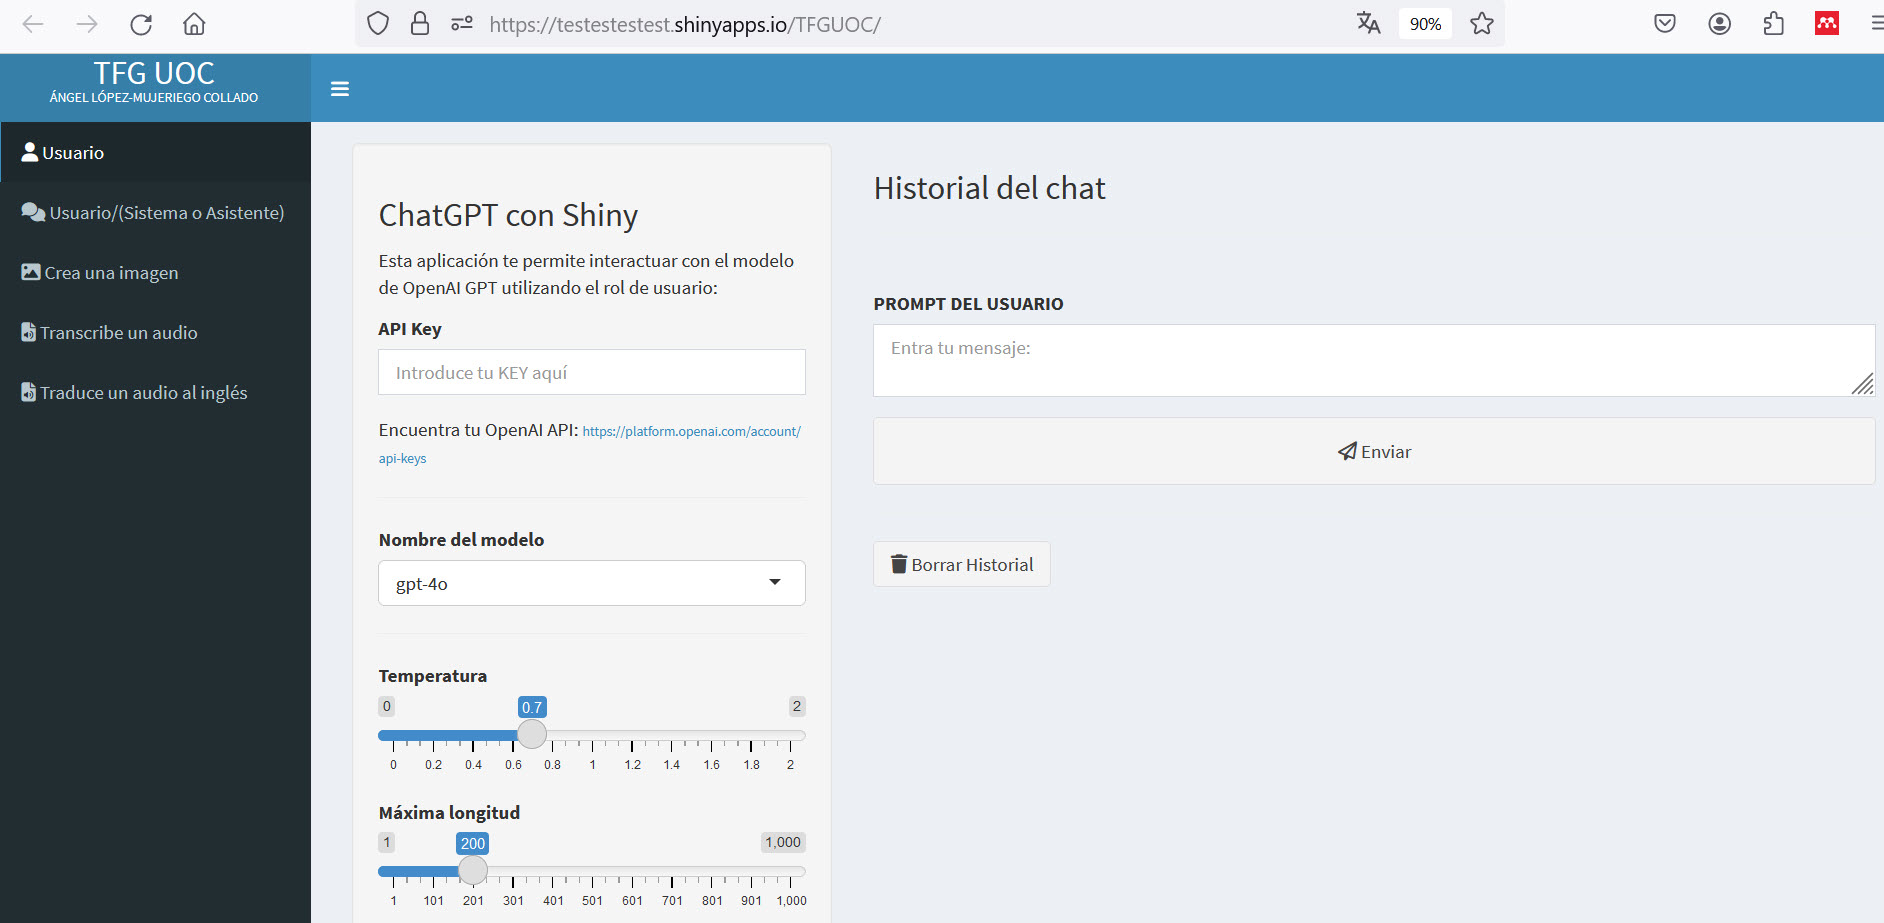
\includegraphics[width=1\linewidth]{FIG2} 

}

\caption{Aplicación de Shiny para interactuar con ChatGPT.}\label{fig:CURSO-1}
\end{figure}

Las 5 aplicaciones creadas se pueden ver en la parte superior izquierda tal y como se muestra en la \ref{fig:CURSO-2}.

\begin{figure}

{\centering 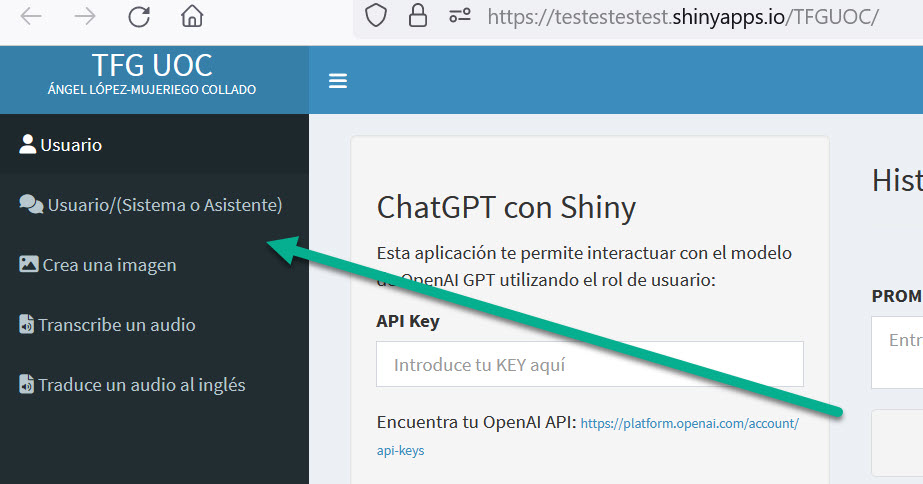
\includegraphics[width=1\linewidth]{FIG3} 

}

\caption{Cinco aplicaciones independientes creadas.}\label{fig:CURSO-2}
\end{figure}

Tal y como se puede ver en la \ref{fig:CURSO-2}, las aplicaciones son las siguientes:

\begin{enumerate}
\def\labelenumi{\arabic{enumi}.}
\tightlist
\item
  Usuario
\item
  Usuario/(Sistema o Asistente)
\item
  Crea una imagen
\item
  Transcribe un audio
\item
  Traduce un audio al inglés
\end{enumerate}

\section{Aplicación Usuario}\label{aplicaciuxf3n-usuario}

Tal y como muestra la \ref{fig:CURSO-3}, esta aplicación permite interactuar con ChatGPT de la que explicaré.

\begin{figure}

{\centering 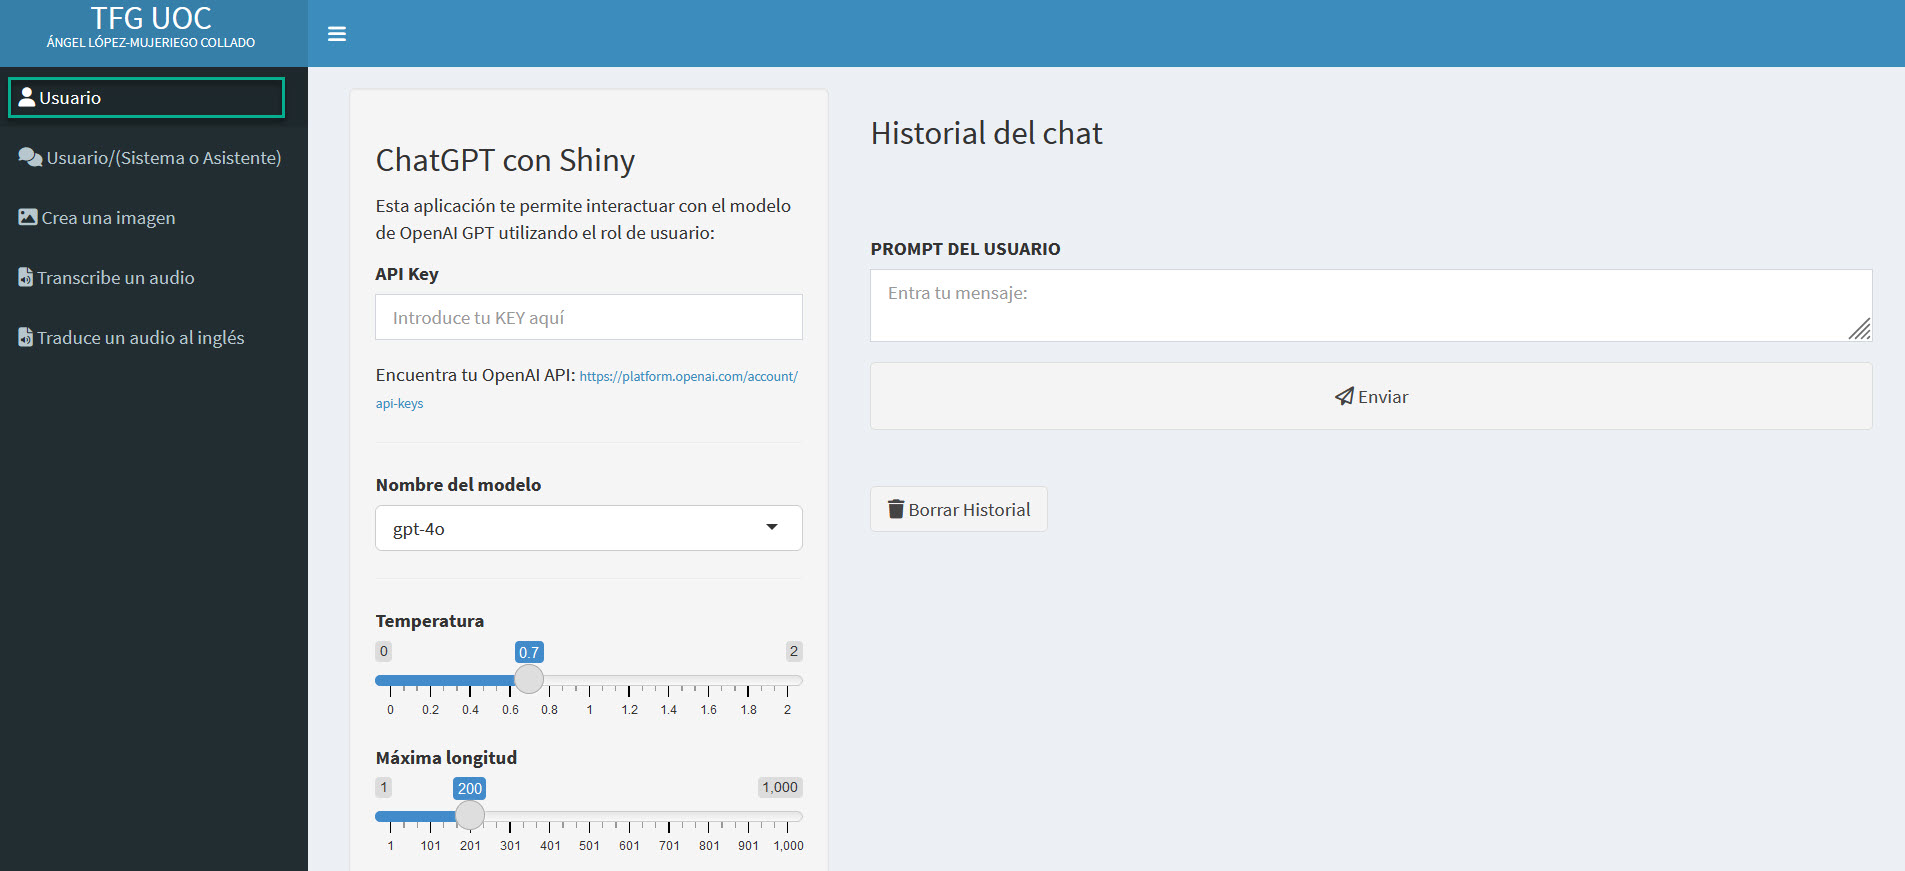
\includegraphics[width=1\linewidth]{FIG4} 

}

\caption{Primera aplicación llamada Usuario.}\label{fig:CURSO-3}
\end{figure}

Primero hace falta introducir la API key (\ref{fig:CURSO-4}) con lo que se debe tener esta llave generada. En el siguiente enlace:

\url{https://platform.openai.com/account/api-keys}

se puede acceder a generarla, guardarla y una vez se ha utilizado en una sesión es recomendable generar una nueva y borrar la anterior (\ref{fig:CURSO-5}).

\begin{figure}

{\centering 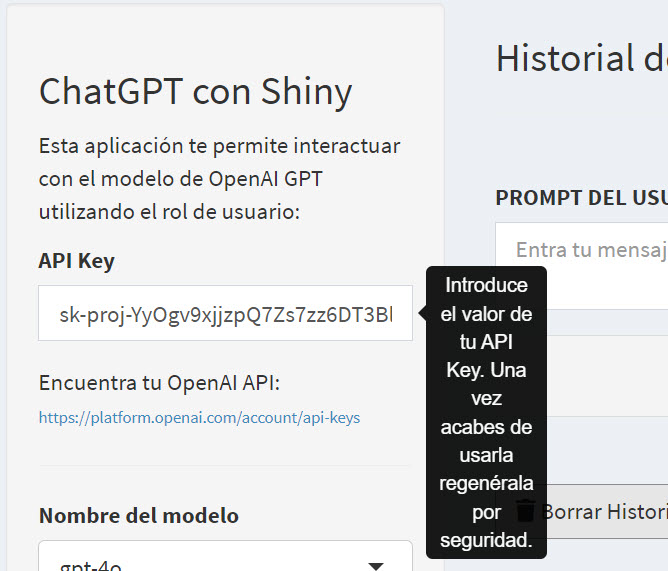
\includegraphics[width=0.6\linewidth]{FIG5} 

}

\caption{Introducción de a la API Key en la aplicación.}\label{fig:CURSO-4}
\end{figure}

\begin{figure}

{\centering 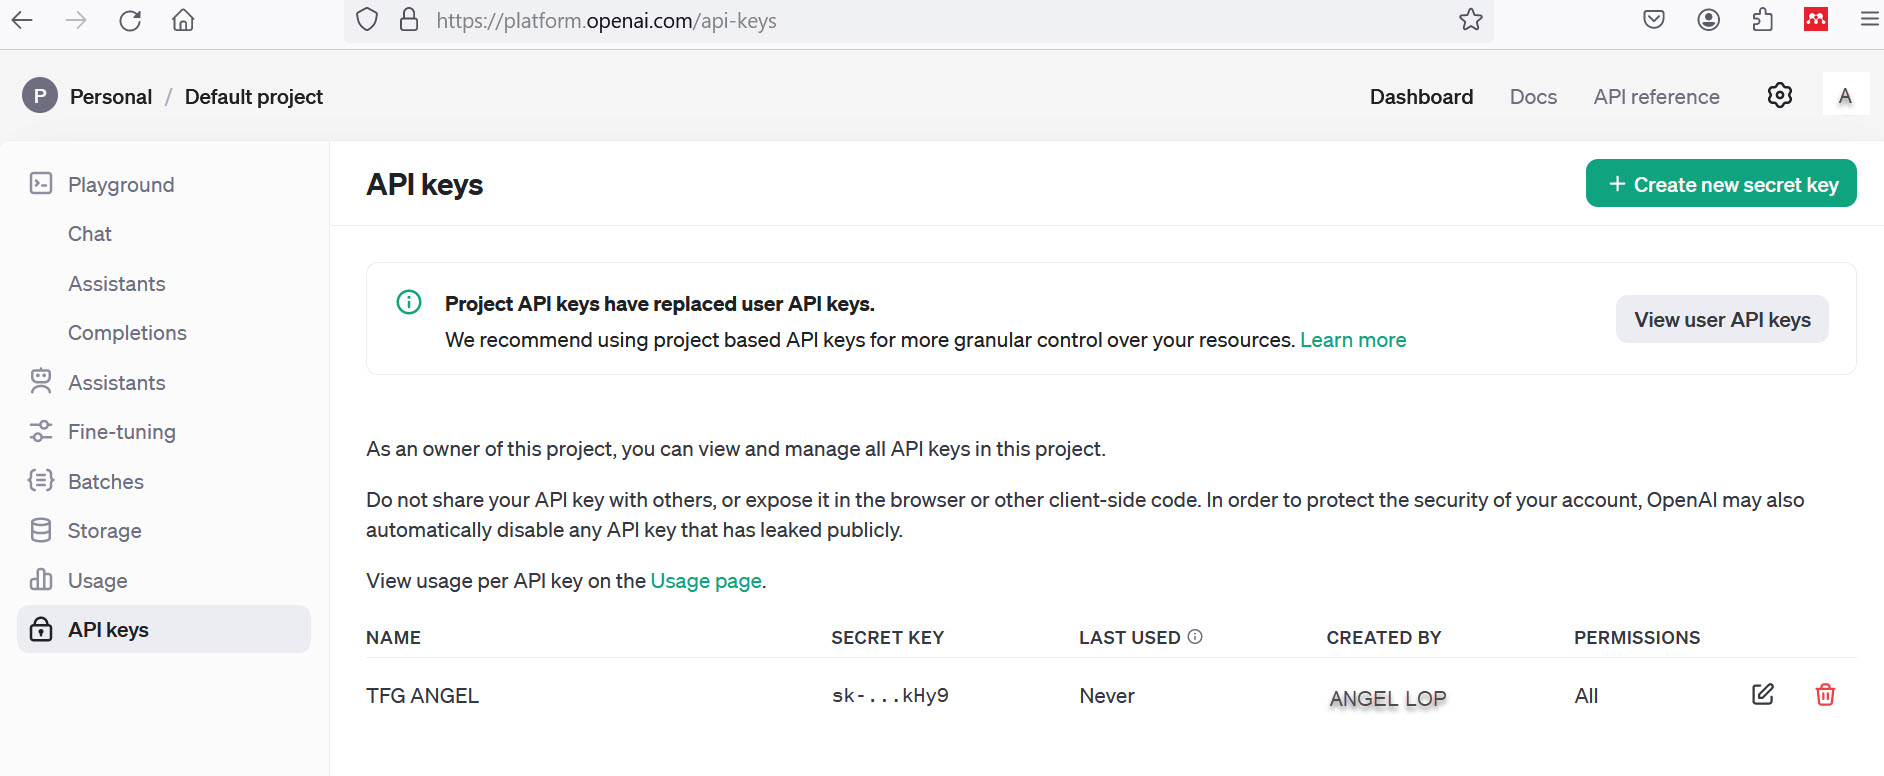
\includegraphics[width=1\linewidth]{FIG6} 

}

\caption{Generación de la API Key en la web oficial de OpenAI. }\label{fig:CURSO-5}
\end{figure}

El siguiente paso es escoger el tipo de modelo entrenado por OpenAI y tenemos 3 posibilidades en este caso, el más reciente, gpt-4o, seguido de gpt-4-turbo y gpt-3.5-turbo tal y como se puede ver en la \ref{fig:CURSO-6}.

\begin{figure}

{\centering 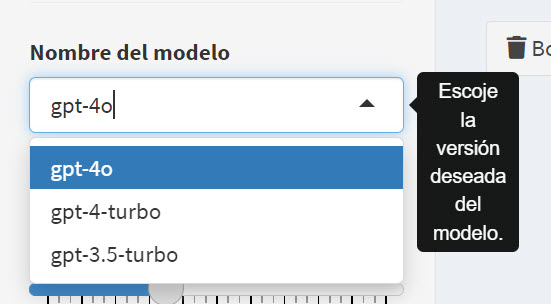
\includegraphics[width=0.6\linewidth]{FIG7} 

}

\caption{Modelos disponibles  de OpenAI en la aplicación.}\label{fig:CURSO-6}
\end{figure}

En la \ref{fig:CURSO-7} se muestran los valores disponibles para la variable Temperatura, siendo 0 un valor faltado de aleatoriedad y más predecible y siendo 1 o más valores que generan texto con mayor variedad y creatividad. Dependiendo de lo que se necesite se va escoger el valor que se crea oportuno.

\begin{figure}

{\centering 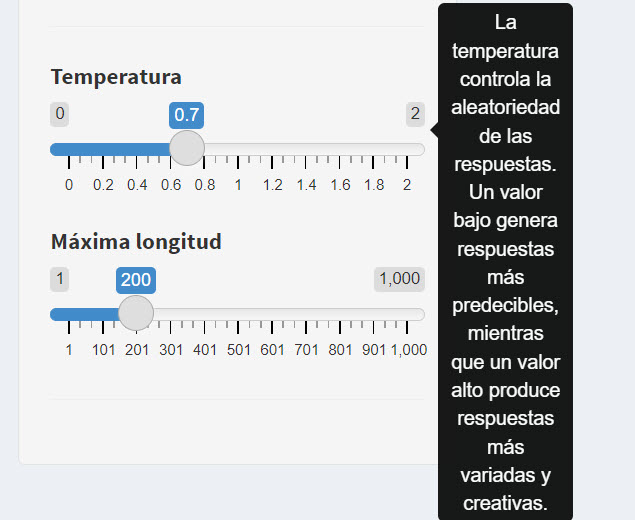
\includegraphics[width=0.6\linewidth]{FIG8} 

}

\caption{Valores de la temperatura disponible para el modelo.}\label{fig:CURSO-7}
\end{figure}

En la \ref{fig:CURSO-8} se muestra donde se puedes escoger la longitud del texto generado variando desde 1 token a 1000 tokens.

\begin{figure}

{\centering 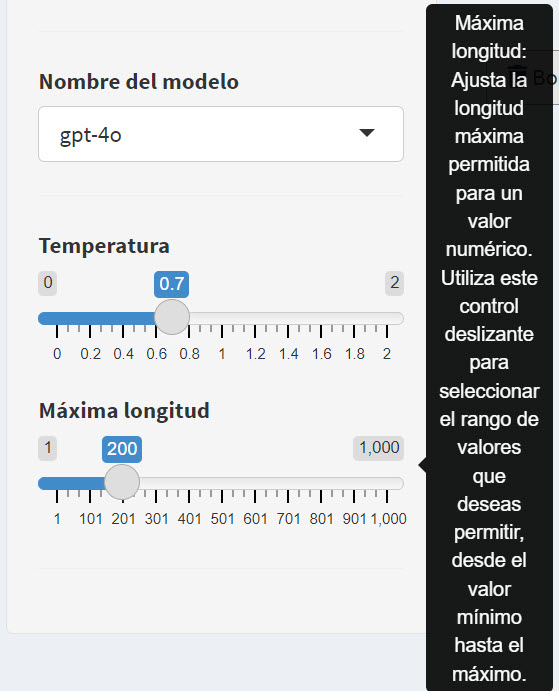
\includegraphics[width=0.6\linewidth]{FIG9} 

}

\caption{Número de tokens escogido como longitud de la respuesta de 1 a 1000.}\label{fig:CURSO-8}
\end{figure}

En la \ref{fig:CURSO-9} se encuentra la parte en la que se encuentra el chat con la posibilidad de introducir el texto pregunta, con el botón enviar y el botón borrar historial cuando se desee.

\begin{figure}

{\centering 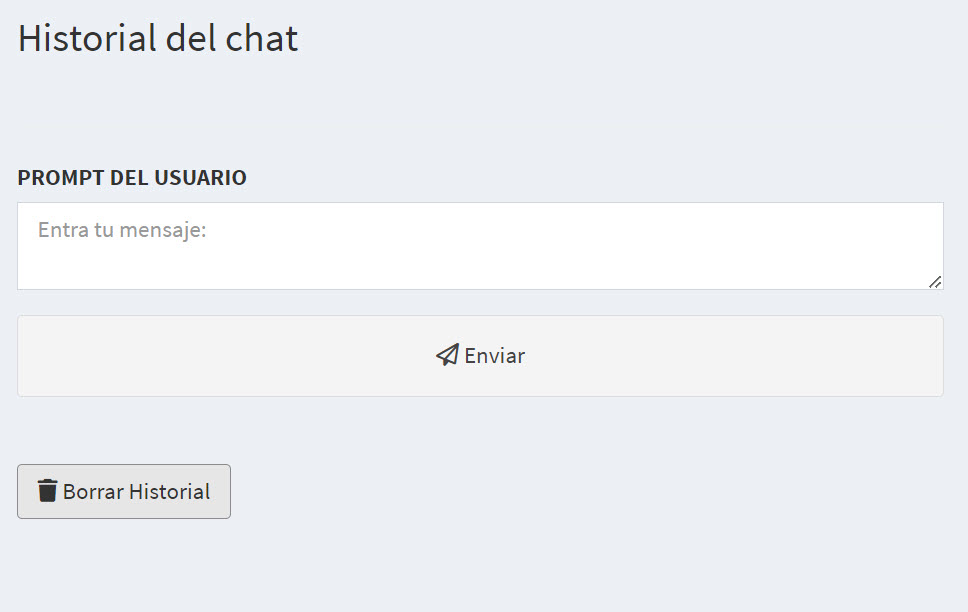
\includegraphics[width=0.6\linewidth]{FIG10} 

}

\caption{Historial del Chat, introducción del texto, botón de enviar y botón de borrar historial.}\label{fig:CURSO-9}
\end{figure}

En la \ref{fig:CURSO-10} se muestra un ejemplo sencillo en el que se pregunta ``¿Cuál es la capital de Cataluña?'' y la aplicación responde en el área verde ``Claro, la capital de Cataluña es Barcelona. Es una ciudad conocida por su arquitecura, cultura y vibrante vida urbana''. Y debajo aparece de nuevo el pompt del usuario para poder seguir interactuando.

\begin{figure}

{\centering 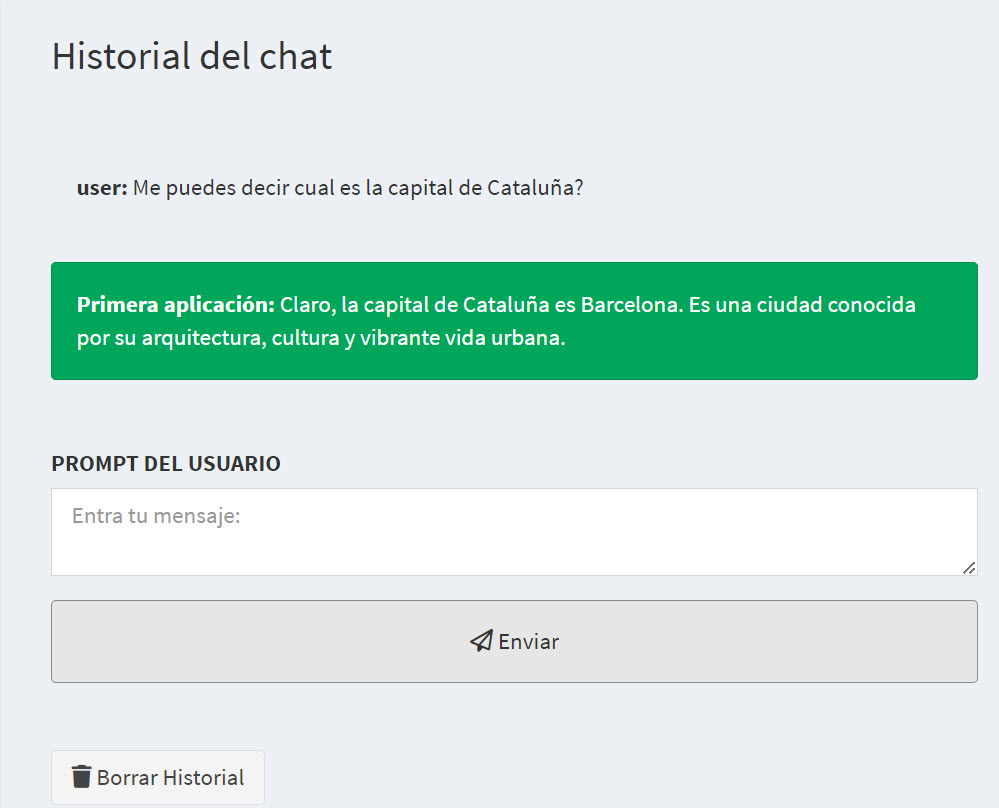
\includegraphics[width=0.6\linewidth]{FIG11} 

}

\caption{Ejemplo de uso del chat de la aplicación.}\label{fig:CURSO-10}
\end{figure}

\section{Aplicación Usuario/(Sistema o Asistente)}\label{aplicaciuxf3n-usuariosistema-o-asistente}

En la \ref{fig:CURSO-11} se muestra la segunda aplicación llamada Usuario/(Sistema o Asistente) y que es igual que la anterior con la diferencia de que hay un espacio llamado ``SISTEMA DE PROMPT'' donde el usuario tiene la opción de utilizar dos roles, el de usuario y el de sitema. Ya veremos más adelante como se puede utilizar de forma eficiente.

\begin{figure}

{\centering 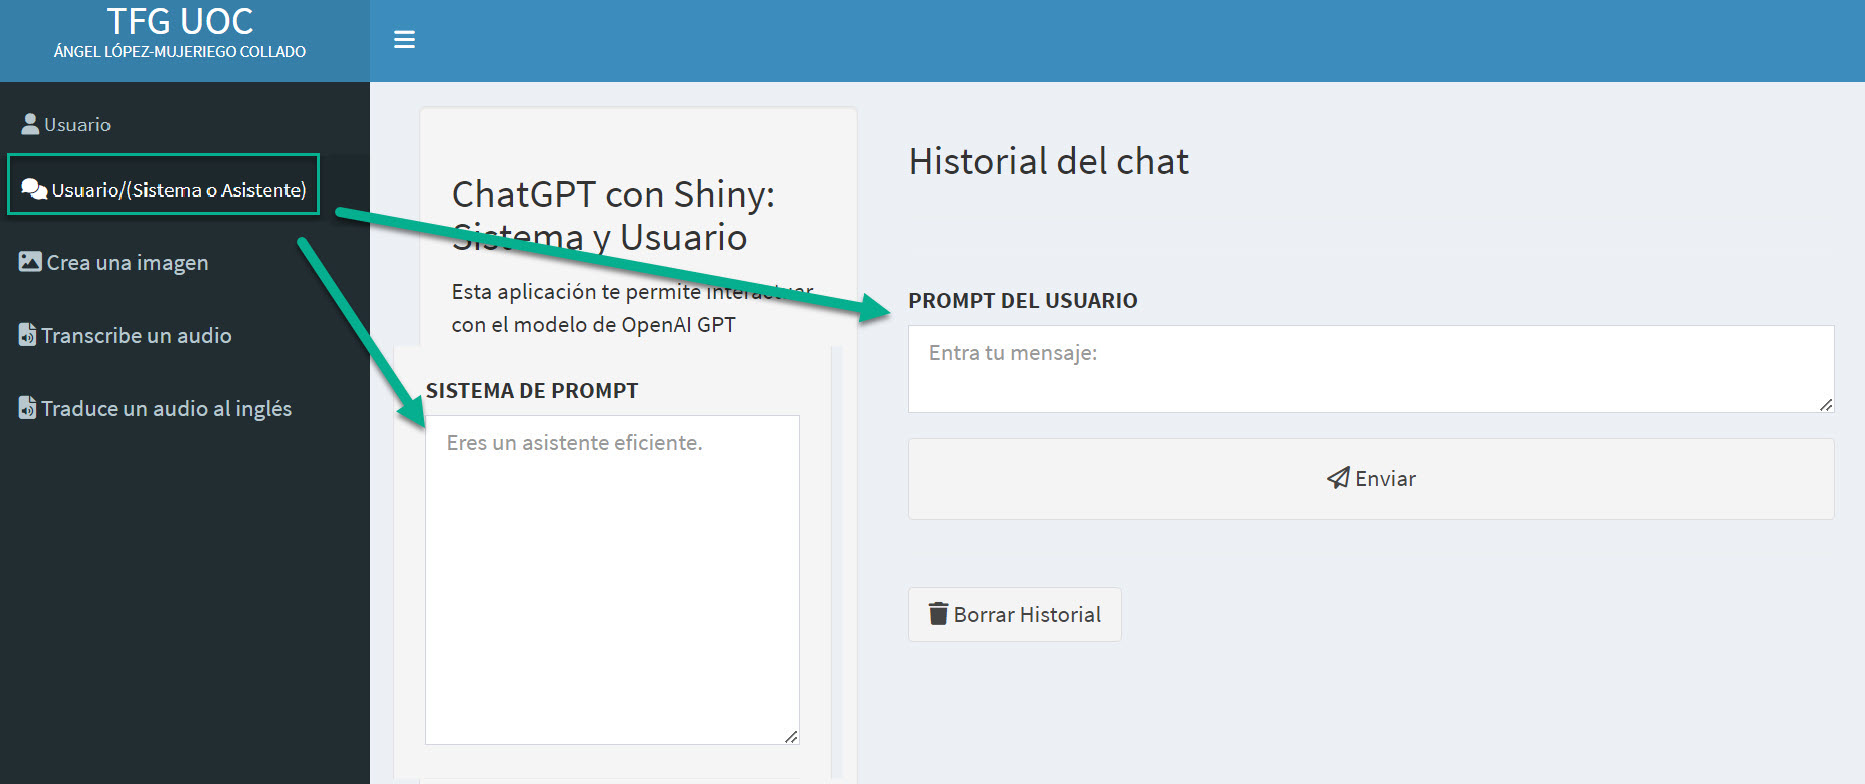
\includegraphics[width=0.6\linewidth]{FIG12} 

}

\caption{Aplicación Usuario/(Sistema o Asistente) en la que se añade el sistema de prompt.}\label{fig:CURSO-11}
\end{figure}

En la \ref{fig:CURSO-12} se puede ver como en el sistema de prompt se ha especificado que realice respuestas solo si son de deporte y que de lo contrario indique que solo contesta a este tipo de preguntas. En cambio, cuando se le pregunta ¿Qué es el fútbol? Responde claramente.

\begin{figure}

{\centering 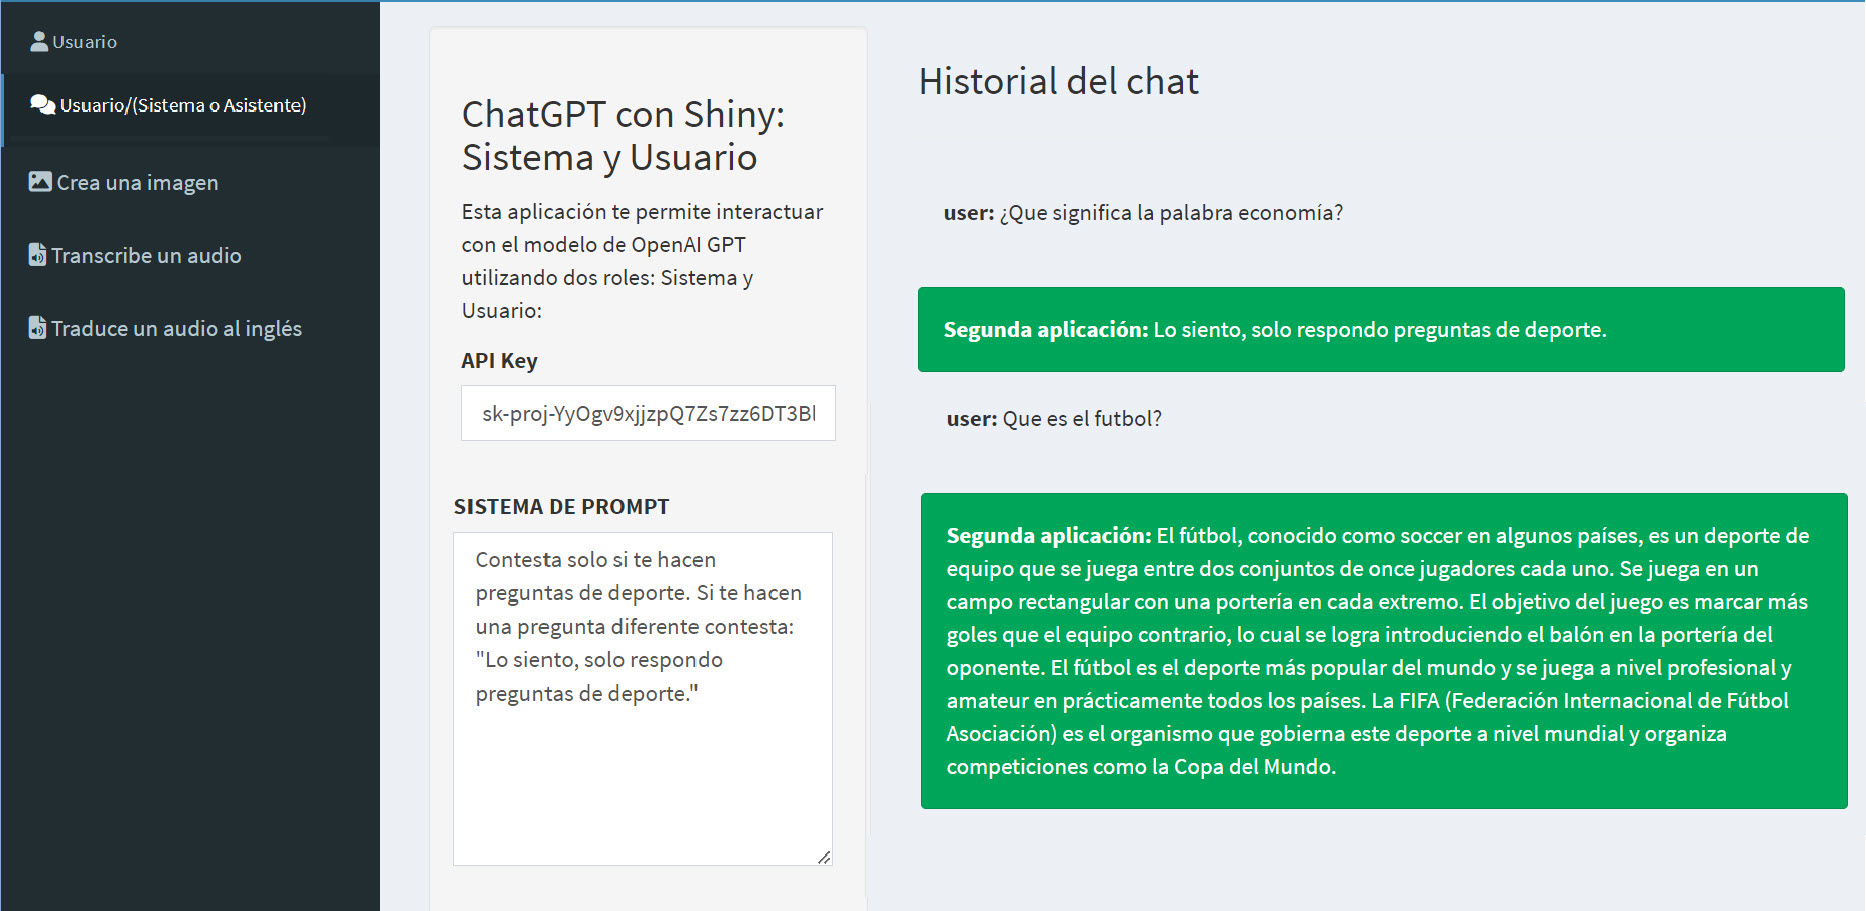
\includegraphics[width=0.6\linewidth]{FIG13} 

}

\caption{Aplicación Usuario/(Sistema o Asistente) en la que se añade el sistema de prompt.}\label{fig:CURSO-12}
\end{figure}

\section{Aplicación Crea una imagen}\label{aplicaciuxf3n-crea-una-imagen}

La siguiente aplicación se llama ``Crea una imagen'' (\ref{fig:CURSO-13}) y a partir de la introducción de una propuesta en el área correspondiente y despues de clicar en el boton ``Genera Imagen'' la imagen se genera. Esta aplicación solo se puede ejecutar si previamente se han usado la primera o la segunda, ya que estas útlimas guardan la API Key en el sistema y ya no hace falta introducirla de nuevo.

\begin{figure}

{\centering 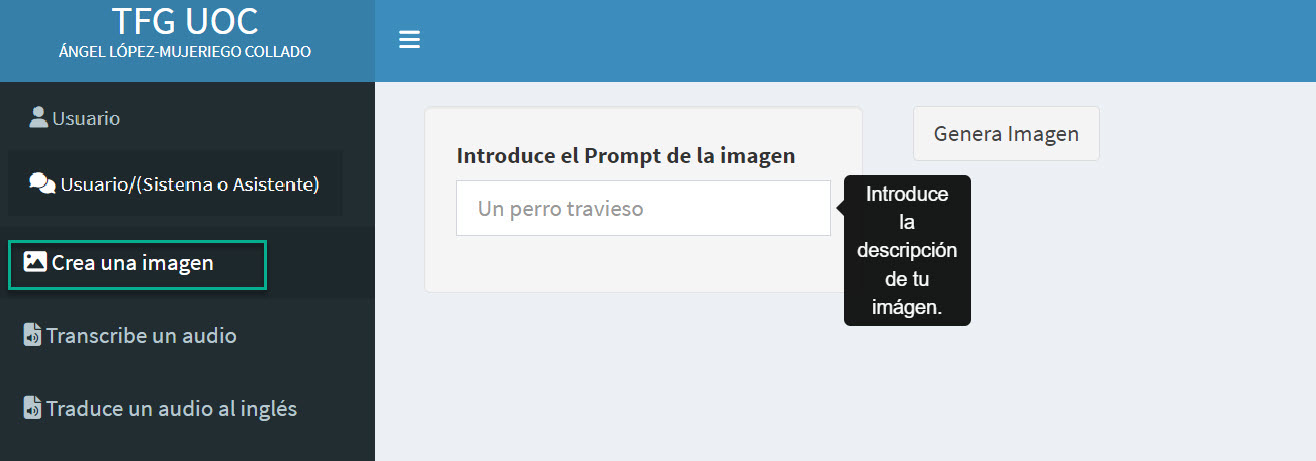
\includegraphics[width=0.6\linewidth]{FIG14} 

}

\caption{Aplicación Crea una imagen.}\label{fig:CURSO-13}
\end{figure}

Se observa en la \ref{fig:CURSO-14} como se ha generado una puesta de sol tal y como se había pedido. También se observa que las imágenes siempre son fotografías ya existentes, es decir, no está utilizando Dall-E 3, sino que reutiliza imágenes de algún repositorio disponible.

\begin{figure}

{\centering 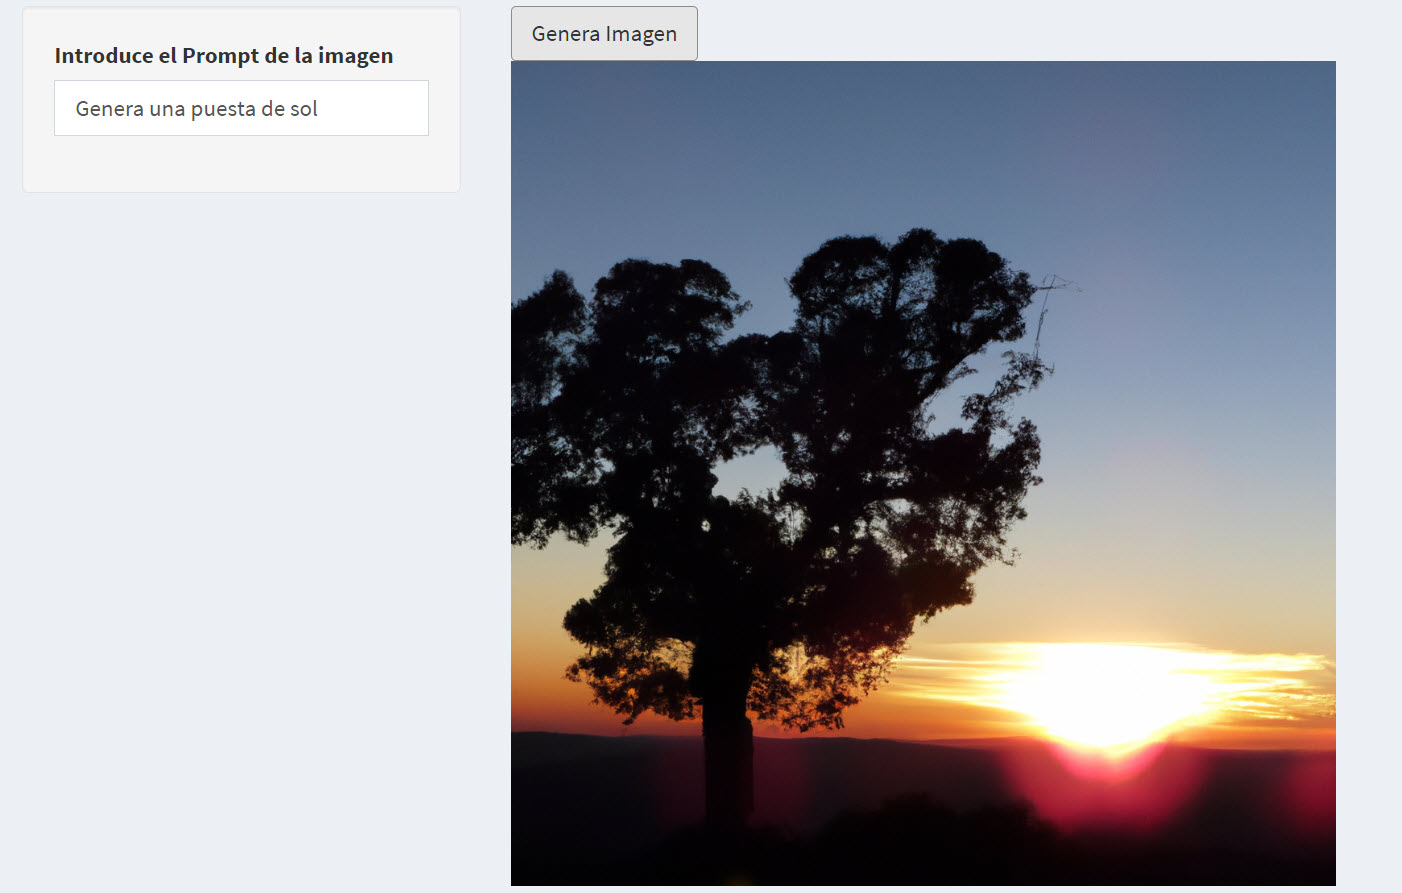
\includegraphics[width=0.6\linewidth]{FIG15} 

}

\caption{Uso de la Aplicación Crea una imagen para generar una puesta de sol.}\label{fig:CURSO-14}
\end{figure}

\chapter{Conclusion}\label{conclusion}

Este es el tfg de Ángel López-Mujeriego Collado.

  \bibliography{book.bib,packages.bib}

\end{document}
